\section{Conceptual Modeling}

The next step after requirement analysis is conceptual modeling. Conceptual modeling is the process of developing an abstract model or graphical representation using real-world concepts or ideas. It is a high-level diagram that defines, describes, organizes, and presents data elements and their relationships with relatively few details. 

For this project, the Entity Relationship Model (ERM) was chosen as it is widely used and was emphasized in our course. ERM provides a clear and organized way to represent data structures, which is essential for the campus event management system.

\subsection{Entity-Relationship Model}

An Entity-Relationship Diagram (ERD) shows the relationships of entities stored in a database. ER diagrams explain the logical structure of a database and illustrate how entities interact. In ER diagrams, three basic concepts are used:

\begin{enumerate}
    \item \textbf{Entity}: In database management systems, an entity is a data object that represents a real-world object or concept, such as an event or a participant. Entities are often represented as tables, with each row representing a specific instance. Entities are shown in rectangular shapes in the ER model.

    \item \textbf{Attribute}: An attribute represents a characteristic or property of an entity. For example, attributes for an event entity might include \textit{event name}, \textit{date}, and \textit{location}. Attributes are represented by oval shapes in the ER model.

    \item \textbf{Relationship}: Relationships are connections between entities that define how data in one entity relates to data in another. In the ER diagram, relationships between entities are represented by diamonds and are labeled to describe the interaction. Common types of relationships include:
    \begin{enumerate}
        \item One-to-One
        \item One-to-Many
        \item Many-to-One
        \item Many-to-Many
    \end{enumerate}
\end{enumerate}

\subsection{Detailing the Entity-Relationship Model}

From the analysis, the following entities and relationships have been identified for the Campus Event Management System:

\subsubsection{Entity Types}

\begin{enumerate}
    \item \textbf{User}: Represents users of the system with attributes such as \textit{user\_id}, \textit{username}, \textit{email}, \textit{password}, \textit{user\_type}, \textit{created\_at}, and \textit{last\_login}.
    \item \textbf{Event}: Represents each campus event, including attributes like \textit{event\_id}, \textit{event\_name}, \textit{description}, \textit{event\_date}, \textit{start\_time}, \textit{end\_time}, \textit{location\_id}, \textit{organizer\_id}, \textit{status}, and \textit{max\_attendees}.
    \item \textbf{Organizer}: Represents individuals organizing events with attributes such as \textit{organizer\_id}, \textit{name}, \textit{contact\_number}, \textit{email}, \textit{user\_id}, and \textit{organization}.
    \item \textbf{Participant}: Represents people attending events, including attributes like \textit{participant\_id}, \textit{event\_id}, \textit{user\_id}, \textit{registration\_date}, and \textit{status}.
    \item \textbf{Location}: Represents locations where events are held, with attributes like \textit{location\_id}, \textit{room\_name}, \textit{building}, \textit{capacity}, and \textit{availability\_status}.
    % \item \textbf{Resource}: Represents resources allocated for events, including attributes like \textit{resource\_id}, \textit{resource\_type}, \textit{quantity}, \textit{availability\_status}, and \textit{location\_id}.
    % \item \textbf{Booking}: Represents the booking of locations and resources, with attributes like \textit{booking\_id}, \textit{event\_id}, \textit{location\_id}, \textit{resource\_id}, \textit{start\_time}, and \textit{end\_time}.
    % \item \textbf{Notification}: Represents notifications sent to users with attributes like \textit{notification\_id}, \textit{user\_id}, \textit{event\_id}, \textit{message}, \textit{notification\_date}, and \textit{status}.
\end{enumerate}

\subsubsection{Relationship Types}

The relationships between the entities identified in the ER model are as follows:

\begin{itemize}
    \item \textbf{Organizes}: Connects \textit{Organizer} and \textit{Event} entities, where each organizer can manage multiple events.
    \item \textbf{Registers}: Connects \textit{Participant} and \textit{Event} entities, where a participant can register for multiple events, and each event can have multiple participants.
    \item \textbf{Requires}: Connects \textit{Event} and \textit{Resource} entities, where an event may require multiple resources, and each resource can be allocated to multiple events.
    \item \textbf{Located At}: Connects \textit{Event} and \textit{Location} entities, where each event is held in a specified location.
\end{itemize}
\begin{figure}[h]
    \centering
    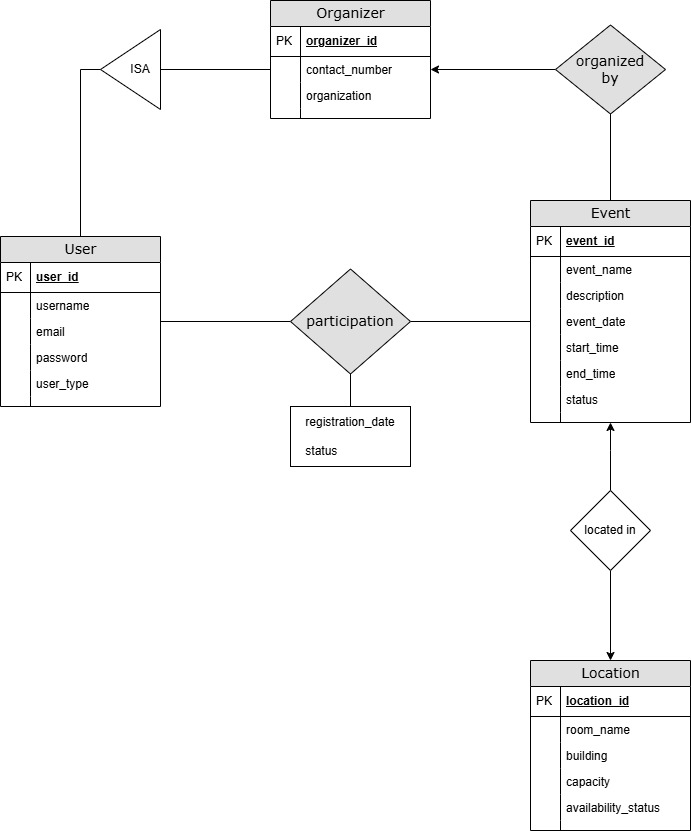
\includegraphics[scale=0.4]{graphics/Event_Management.jpg}
\end{figure}
In the figure the ER diagram displays these entity types and their relationships. For instance, the relationship between \textbf{Event} and \textbf{Participant} indicates that one participant can register for multiple events. The \textbf{Organizer} manages one or more events, and resources are allocated to events as needed.

Entities are represented in rectangular shapes, relationships in diamond shapes, and attributes in oval shapes.
